

\tikzset{every picture/.style={line width=0.75pt}} %set default line width to 0.75pt        

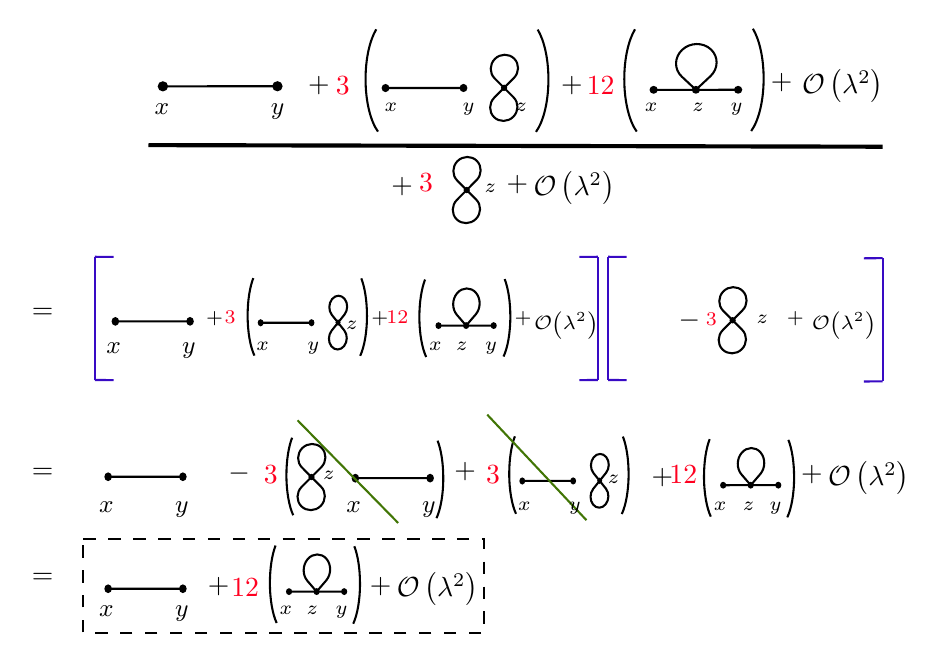
\begin{tikzpicture}[x=0.75pt,y=0.75pt,yscale=-1,xscale=1]
%uncomment if require: \path (0,671); %set diagram left start at 0, and has height of 671

%Shape: Tear Drop [id:dp18661306967885327] 
\draw   (433.64,43.56) .. controls (433.64,43.56) and (433.64,43.56) .. (433.64,43.56) .. controls (429.88,40.05) and (429.97,34.26) .. (433.85,30.64) .. controls (437.72,27.02) and (443.91,26.93) .. (447.67,30.44) .. controls (451.42,33.95) and (451.33,39.74) .. (447.45,43.36) .. controls (442.78,47.73) and (440.43,49.92) .. (440.44,49.92) .. controls (440.43,49.92) and (438.17,47.81) .. (433.64,43.56) -- cycle ;
%Shape: Ellipse [id:dp9361439189202535] 
\draw  [fill={rgb, 255:red, 0; green, 0; blue, 0 }  ,fill opacity=1 ] (438.99,49.92) .. controls (438.99,49.17) and (439.64,48.56) .. (440.44,48.56) .. controls (441.24,48.56) and (441.89,49.17) .. (441.89,49.92) .. controls (441.89,50.67) and (441.24,51.27) .. (440.44,51.27) .. controls (439.64,51.27) and (438.99,50.67) .. (438.99,49.92) -- cycle ;
%Straight Lines [id:da6065723003123908] 
\draw    (420.09,49.93) -- (460.79,49.91) ;
%Shape: Ellipse [id:dp03103763323336939] 
\draw  [fill={rgb, 255:red, 0; green, 0; blue, 0 }  ,fill opacity=1 ] (418.64,49.93) .. controls (418.64,49.18) and (419.29,48.57) .. (420.09,48.57) .. controls (420.89,48.57) and (421.54,49.18) .. (421.54,49.93) .. controls (421.54,50.68) and (420.89,51.29) .. (420.09,51.29) .. controls (419.29,51.29) and (418.64,50.68) .. (418.64,49.93) -- cycle ;
%Shape: Ellipse [id:dp66623428202012] 
\draw  [fill={rgb, 255:red, 0; green, 0; blue, 0 }  ,fill opacity=1 ] (459.34,49.91) .. controls (459.34,49.16) and (459.99,48.55) .. (460.79,48.55) .. controls (461.59,48.55) and (462.24,49.16) .. (462.24,49.91) .. controls (462.24,50.66) and (461.59,51.26) .. (460.79,51.26) .. controls (459.99,51.26) and (459.34,50.66) .. (459.34,49.91) -- cycle ;
%Straight Lines [id:da724517629051785] 
\draw [line width=1.5]    (176.71,76.57) -- (530.38,77.34) ;
%Shape: Tear Drop [id:dp6761845216588682] 
\draw   (343.45,44.38) .. controls (340.92,41.84) and (340.98,37.66) .. (343.59,35.04) .. controls (346.2,32.42) and (350.37,32.36) .. (352.9,34.9) .. controls (355.43,37.44) and (355.36,41.61) .. (352.75,44.23) .. controls (349.6,47.39) and (348.03,48.97) .. (348.03,48.97) .. controls (348.03,48.97) and (346.5,47.44) .. (343.45,44.38) -- cycle ;
%Shape: Tear Drop [id:dp8902749219969582] 
\draw   (352.61,53.57) .. controls (352.61,53.57) and (352.61,53.57) .. (352.61,53.57) .. controls (355.14,56.11) and (355.08,60.29) .. (352.47,62.91) .. controls (349.86,65.53) and (345.69,65.59) .. (343.16,63.05) .. controls (340.63,60.51) and (340.69,56.33) .. (343.3,53.72) .. controls (346.45,50.55) and (348.03,48.97) .. (348.03,48.98) .. controls (348.03,48.97) and (349.56,50.51) .. (352.61,53.57) -- cycle ;
%Shape: Ellipse [id:dp5450651522816483] 
\draw  [fill={rgb, 255:red, 0; green, 0; blue, 0 }  ,fill opacity=1 ] (347.05,48.97) .. controls (347.05,48.43) and (347.49,47.99) .. (348.03,47.99) .. controls (348.57,47.99) and (349.01,48.43) .. (349.01,48.97) .. controls (349.01,49.52) and (348.57,49.96) .. (348.03,49.96) .. controls (347.49,49.96) and (347.05,49.52) .. (347.05,48.97) -- cycle ;
%Straight Lines [id:da2540200515480916] 
\draw    (183.64,48.24) -- (238.82,48.21) ;
%Shape: Ellipse [id:dp8276270069093603] 
\draw  [fill={rgb, 255:red, 0; green, 0; blue, 0 }  ,fill opacity=1 ] (181.67,48.24) .. controls (181.67,47.18) and (182.55,46.33) .. (183.64,46.33) .. controls (184.72,46.33) and (185.6,47.18) .. (185.6,48.24) .. controls (185.6,49.3) and (184.72,50.16) .. (183.64,50.16) .. controls (182.55,50.16) and (181.67,49.3) .. (181.67,48.24) -- cycle ;
%Shape: Ellipse [id:dp28106669465315004] 
\draw  [fill={rgb, 255:red, 0; green, 0; blue, 0 }  ,fill opacity=1 ] (236.85,48.21) .. controls (236.85,47.15) and (237.73,46.29) .. (238.82,46.29) .. controls (239.91,46.29) and (240.79,47.15) .. (240.79,48.21) .. controls (240.79,49.27) and (239.91,50.13) .. (238.82,50.13) .. controls (237.73,50.13) and (236.85,49.27) .. (236.85,48.21) -- cycle ;
%Straight Lines [id:da755227783850173] 
\draw    (290.91,49.07) -- (328.48,49.04) ;
%Shape: Ellipse [id:dp45408460837764897] 
\draw  [fill={rgb, 255:red, 0; green, 0; blue, 0 }  ,fill opacity=1 ] (289.57,49.07) .. controls (289.57,48.28) and (290.17,47.65) .. (290.91,47.65) .. controls (291.65,47.65) and (292.25,48.28) .. (292.25,49.07) .. controls (292.25,49.85) and (291.65,50.49) .. (290.91,50.49) .. controls (290.17,50.49) and (289.57,49.85) .. (289.57,49.07) -- cycle ;
%Shape: Ellipse [id:dp9026279693874513] 
\draw  [fill={rgb, 255:red, 0; green, 0; blue, 0 }  ,fill opacity=1 ] (327.14,49.04) .. controls (327.14,48.26) and (327.74,47.62) .. (328.48,47.62) .. controls (329.22,47.62) and (329.82,48.26) .. (329.82,49.04) .. controls (329.82,49.83) and (329.22,50.47) .. (328.48,50.47) .. controls (327.74,50.47) and (327.14,49.83) .. (327.14,49.04) -- cycle ;
%Shape: Arc [id:dp15498338520509913] 
\draw  [draw opacity=0] (287.27,70.05) .. controls (283.7,65.11) and (281.29,55.65) .. (281.29,44.79) .. controls (281.29,34.78) and (283.34,25.96) .. (286.45,20.77) -- (292.95,44.79) -- cycle ; \draw   (287.27,70.05) .. controls (283.7,65.11) and (281.29,55.65) .. (281.29,44.79) .. controls (281.29,34.78) and (283.34,25.96) .. (286.45,20.77) ;  
%Shape: Arc [id:dp4714525605138319] 
\draw  [draw opacity=0] (363.4,70.19) .. controls (366.97,65.25) and (369.39,55.79) .. (369.39,44.93) .. controls (369.39,34.92) and (367.34,26.1) .. (364.22,20.91) -- (357.72,44.93) -- cycle ; \draw   (363.4,70.19) .. controls (366.97,65.25) and (369.39,55.79) .. (369.39,44.93) .. controls (369.39,34.92) and (367.34,26.1) .. (364.22,20.91) ;  
%Shape: Arc [id:dp16860763876835982] 
\draw  [draw opacity=0] (411.93,70.05) .. controls (408.36,65.11) and (405.94,55.65) .. (405.94,44.79) .. controls (405.94,34.78) and (407.99,25.96) .. (411.11,20.77) -- (417.61,44.79) -- cycle ; \draw   (411.93,70.05) .. controls (408.36,65.11) and (405.94,55.65) .. (405.94,44.79) .. controls (405.94,34.78) and (407.99,25.96) .. (411.11,20.77) ;  
%Shape: Arc [id:dp8308055291472114] 
\draw  [draw opacity=0] (467.09,69.78) .. controls (470.66,64.83) and (473.08,55.37) .. (473.08,44.51) .. controls (473.08,34.5) and (471.03,25.68) .. (467.91,20.49) -- (461.41,44.51) -- cycle ; \draw   (467.09,69.78) .. controls (470.66,64.83) and (473.08,55.37) .. (473.08,44.51) .. controls (473.08,34.5) and (471.03,25.68) .. (467.91,20.49) ;  
%Shape: Tear Drop [id:dp0009791639330052337] 
\draw   (325.44,93.62) .. controls (325.44,93.62) and (325.44,93.62) .. (325.44,93.62) .. controls (325.44,93.62) and (325.44,93.62) .. (325.44,93.62) .. controls (322.91,91.08) and (322.97,86.9) .. (325.58,84.28) .. controls (328.19,81.66) and (332.36,81.6) .. (334.89,84.14) .. controls (337.42,86.68) and (337.36,90.86) .. (334.75,93.47) .. controls (331.59,96.63) and (330.02,98.21) .. (330.02,98.21) .. controls (330.02,98.21) and (328.49,96.68) .. (325.44,93.62) -- cycle ;
%Shape: Tear Drop [id:dp804378575754482] 
\draw   (334.6,102.81) .. controls (334.6,102.81) and (334.6,102.81) .. (334.6,102.81) .. controls (337.13,105.35) and (337.07,109.53) .. (334.46,112.15) .. controls (331.85,114.77) and (327.68,114.83) .. (325.15,112.29) .. controls (322.62,109.75) and (322.69,105.57) .. (325.3,102.96) .. controls (328.44,99.79) and (330.02,98.22) .. (330.02,98.22) .. controls (330.02,98.22) and (331.55,99.75) .. (334.6,102.81) -- cycle ;
%Shape: Ellipse [id:dp09914460271355052] 
\draw  [fill={rgb, 255:red, 0; green, 0; blue, 0 }  ,fill opacity=1 ] (329.04,98.21) .. controls (329.04,97.67) and (329.48,97.23) .. (330.02,97.23) .. controls (330.56,97.23) and (331,97.67) .. (331,98.21) .. controls (331,98.76) and (330.56,99.2) .. (330.02,99.2) .. controls (329.48,99.2) and (329.04,98.76) .. (329.04,98.21) -- cycle ;
%Shape: Tear Drop [id:dp09610633961756954] 
\draw   (325.3,158.36) .. controls (325.3,158.36) and (325.3,158.36) .. (325.3,158.36) .. controls (322.85,155.51) and (322.91,150.82) .. (325.44,147.88) .. controls (327.97,144.94) and (332,144.86) .. (334.46,147.71) .. controls (336.91,150.57) and (336.85,155.26) .. (334.32,158.2) .. controls (331.26,161.75) and (329.74,163.52) .. (329.74,163.53) .. controls (329.74,163.52) and (328.26,161.8) .. (325.3,158.36) -- cycle ;
%Shape: Ellipse [id:dp3878985059990172] 
\draw  [fill={rgb, 255:red, 0; green, 0; blue, 0 }  ,fill opacity=1 ] (328.79,163.53) .. controls (328.79,162.92) and (329.22,162.43) .. (329.74,162.43) .. controls (330.26,162.43) and (330.69,162.92) .. (330.69,163.53) .. controls (330.69,164.14) and (330.26,164.63) .. (329.74,164.63) .. controls (329.22,164.63) and (328.79,164.14) .. (328.79,163.53) -- cycle ;
%Straight Lines [id:da6361114296859189] 
\draw    (316.46,163.54) -- (343.02,163.52) ;
%Shape: Ellipse [id:dp7692479461640018] 
\draw  [fill={rgb, 255:red, 0; green, 0; blue, 0 }  ,fill opacity=1 ] (315.51,163.54) .. controls (315.51,162.93) and (315.93,162.44) .. (316.46,162.44) .. controls (316.98,162.44) and (317.4,162.93) .. (317.4,163.54) .. controls (317.4,164.15) and (316.98,164.64) .. (316.46,164.64) .. controls (315.93,164.64) and (315.51,164.15) .. (315.51,163.54) -- cycle ;
%Shape: Ellipse [id:dp6910575048020595] 
\draw  [fill={rgb, 255:red, 0; green, 0; blue, 0 }  ,fill opacity=1 ] (342.07,163.52) .. controls (342.07,162.91) and (342.5,162.42) .. (343.02,162.42) .. controls (343.55,162.42) and (343.97,162.91) .. (343.97,163.52) .. controls (343.97,164.13) and (343.55,164.62) .. (343.02,164.62) .. controls (342.5,164.62) and (342.07,164.13) .. (342.07,163.52) -- cycle ;
%Shape: Tear Drop [id:dp359214032441904] 
\draw   (265.04,158.35) .. controls (265.04,158.35) and (265.04,158.35) .. (265.04,158.35) .. controls (265.04,158.35) and (265.04,158.35) .. (265.04,158.35) .. controls (263.39,156.29) and (263.43,152.9) .. (265.14,150.77) .. controls (266.84,148.65) and (269.56,148.6) .. (271.21,150.66) .. controls (272.86,152.72) and (272.82,156.11) .. (271.12,158.24) .. controls (269.06,160.8) and (268.03,162.08) .. (268.03,162.08) .. controls (268.03,162.08) and (267.04,160.85) .. (265.04,158.35) -- cycle ;
%Shape: Tear Drop [id:dp7368643127985692] 
\draw   (271.02,165.82) .. controls (272.67,167.88) and (272.63,171.27) .. (270.93,173.4) .. controls (269.23,175.52) and (266.51,175.58) .. (264.85,173.52) .. controls (263.2,171.46) and (263.24,168.06) .. (264.95,165.94) .. controls (267.01,163.37) and (268.03,162.09) .. (268.03,162.09) .. controls (268.03,162.09) and (269.03,163.33) .. (271.02,165.82) -- cycle ;
%Shape: Ellipse [id:dp08465472646708516] 
\draw  [fill={rgb, 255:red, 0; green, 0; blue, 0 }  ,fill opacity=1 ] (267.39,162.09) .. controls (267.39,161.65) and (267.68,161.29) .. (268.03,161.29) .. controls (268.38,161.29) and (268.67,161.65) .. (268.67,162.09) .. controls (268.67,162.53) and (268.38,162.88) .. (268.03,162.88) .. controls (267.68,162.88) and (267.39,162.53) .. (267.39,162.09) -- cycle ;
%Straight Lines [id:da5232302965034197] 
\draw    (160.72,161.49) -- (196.75,161.47) ;
%Shape: Ellipse [id:dp12506371014609607] 
\draw  [fill={rgb, 255:red, 0; green, 0; blue, 0 }  ,fill opacity=1 ] (159.44,161.49) .. controls (159.44,160.63) and (160.02,159.94) .. (160.72,159.94) .. controls (161.43,159.94) and (162.01,160.63) .. (162.01,161.49) .. controls (162.01,162.35) and (161.43,163.05) .. (160.72,163.05) .. controls (160.02,163.05) and (159.44,162.35) .. (159.44,161.49) -- cycle ;
%Shape: Ellipse [id:dp49112214847540614] 
\draw  [fill={rgb, 255:red, 0; green, 0; blue, 0 }  ,fill opacity=1 ] (195.46,161.47) .. controls (195.46,160.61) and (196.04,159.91) .. (196.75,159.91) .. controls (197.46,159.91) and (198.03,160.61) .. (198.03,161.47) .. controls (198.03,162.32) and (197.46,163.02) .. (196.75,163.02) .. controls (196.04,163.02) and (195.46,162.32) .. (195.46,161.47) -- cycle ;
%Straight Lines [id:da9308092120040908] 
\draw    (230.75,162.16) -- (255.27,162.14) ;
%Shape: Ellipse [id:dp271514177692578] 
\draw  [fill={rgb, 255:red, 0; green, 0; blue, 0 }  ,fill opacity=1 ] (229.87,162.16) .. controls (229.87,161.52) and (230.27,161.01) .. (230.75,161.01) .. controls (231.23,161.01) and (231.62,161.52) .. (231.62,162.16) .. controls (231.62,162.8) and (231.23,163.32) .. (230.75,163.32) .. controls (230.27,163.32) and (229.87,162.8) .. (229.87,162.16) -- cycle ;
%Shape: Ellipse [id:dp9232774627084169] 
\draw  [fill={rgb, 255:red, 0; green, 0; blue, 0 }  ,fill opacity=1 ] (254.4,162.14) .. controls (254.4,161.5) and (254.79,160.99) .. (255.27,160.99) .. controls (255.75,160.99) and (256.14,161.5) .. (256.14,162.14) .. controls (256.14,162.78) and (255.75,163.3) .. (255.27,163.3) .. controls (254.79,163.3) and (254.4,162.78) .. (254.4,162.14) -- cycle ;
%Shape: Arc [id:dp6454262453177982] 
\draw  [draw opacity=0] (227.74,177.98) .. controls (225.76,173.74) and (224.47,166.68) .. (224.47,158.69) .. controls (224.47,151.44) and (225.53,144.96) .. (227.2,140.66) -- (232.08,158.69) -- cycle ; \draw   (227.74,177.98) .. controls (225.76,173.74) and (224.47,166.68) .. (224.47,158.69) .. controls (224.47,151.44) and (225.53,144.96) .. (227.2,140.66) ;  
%Shape: Arc [id:dp7703609779787192] 
\draw  [draw opacity=0] (278.7,178.1) .. controls (280.68,173.86) and (281.97,166.8) .. (281.97,158.8) .. controls (281.97,151.56) and (280.91,145.08) .. (279.24,140.77) -- (274.36,158.8) -- cycle ; \draw   (278.7,178.1) .. controls (280.68,173.86) and (281.97,166.8) .. (281.97,158.8) .. controls (281.97,151.56) and (280.91,145.08) .. (279.24,140.77) ;  
%Shape: Arc [id:dp8610870639334023] 
\draw  [draw opacity=0] (310.5,178.66) .. controls (308.52,174.42) and (307.22,167.36) .. (307.22,159.36) .. controls (307.22,152.12) and (308.29,145.64) .. (309.96,141.33) -- (314.84,159.36) -- cycle ; \draw   (310.5,178.66) .. controls (308.52,174.42) and (307.22,167.36) .. (307.22,159.36) .. controls (307.22,152.12) and (308.29,145.64) .. (309.96,141.33) ;  
%Shape: Arc [id:dp84583472949954] 
\draw  [draw opacity=0] (347.77,178.43) .. controls (349.75,174.19) and (351.04,167.13) .. (351.04,159.14) .. controls (351.04,151.89) and (349.98,145.41) .. (348.31,141.11) -- (343.43,159.14) -- cycle ; \draw   (347.77,178.43) .. controls (349.75,174.19) and (351.04,167.13) .. (351.04,159.14) .. controls (351.04,151.89) and (349.98,145.41) .. (348.31,141.11) ;  
%Straight Lines [id:da10171520989018334] 
\draw [color={rgb, 255:red, 56; green, 10; blue, 196 }  ,draw opacity=1 ]   (150.87,130.37) -- (150.87,189.72) ;
%Straight Lines [id:da3717524892841779] 
\draw [color={rgb, 255:red, 56; green, 10; blue, 196 }  ,draw opacity=1 ]   (159.87,189.78) -- (150.87,189.72) ;
%Straight Lines [id:da26500998853188584] 
\draw [color={rgb, 255:red, 56; green, 10; blue, 196 }  ,draw opacity=1 ]   (159.87,130.42) -- (150.87,130.37) ;

%Straight Lines [id:da9090241724098136] 
\draw [color={rgb, 255:red, 56; green, 10; blue, 196 }  ,draw opacity=1 ]   (393.26,130.37) -- (393.26,189.72) ;
%Straight Lines [id:da7418346126869394] 
\draw [color={rgb, 255:red, 56; green, 10; blue, 196 }  ,draw opacity=1 ]   (384.26,189.78) -- (393.26,189.72) ;
%Straight Lines [id:da3927715120037272] 
\draw [color={rgb, 255:red, 56; green, 10; blue, 196 }  ,draw opacity=1 ]   (384.26,130.42) -- (393.26,130.37) ;

%Shape: Tear Drop [id:dp5999663033501414] 
\draw   (453.56,156.35) .. controls (453.56,156.35) and (453.56,156.35) .. (453.56,156.35) .. controls (451.03,153.81) and (451.1,149.63) .. (453.7,147.01) .. controls (456.31,144.39) and (460.48,144.33) .. (463.01,146.87) .. controls (465.54,149.41) and (465.48,153.59) .. (462.87,156.2) .. controls (459.71,159.36) and (458.14,160.94) .. (458.14,160.94) .. controls (458.14,160.94) and (456.62,159.41) .. (453.56,156.35) -- cycle ;
%Shape: Tear Drop [id:dp43523696161940095] 
\draw   (462.72,165.54) .. controls (465.25,168.08) and (465.19,172.26) .. (462.58,174.88) .. controls (459.97,177.5) and (455.8,177.56) .. (453.27,175.02) .. controls (450.74,172.48) and (450.81,168.3) .. (453.42,165.69) .. controls (456.56,162.53) and (458.14,160.95) .. (458.14,160.95) .. controls (458.14,160.95) and (459.67,162.48) .. (462.72,165.54) -- cycle ;
%Shape: Ellipse [id:dp6986768159205009] 
\draw  [fill={rgb, 255:red, 0; green, 0; blue, 0 }  ,fill opacity=1 ] (457.17,160.94) .. controls (457.17,160.4) and (457.6,159.96) .. (458.14,159.96) .. controls (458.68,159.96) and (459.12,160.4) .. (459.12,160.94) .. controls (459.12,161.49) and (458.68,161.93) .. (458.14,161.93) .. controls (457.6,161.93) and (457.17,161.49) .. (457.17,160.94) -- cycle ;
%Straight Lines [id:da1788375246822438] 
\draw [color={rgb, 255:red, 56; green, 10; blue, 196 }  ,draw opacity=1 ]   (398.11,130.37) -- (398.11,189.72) ;
%Straight Lines [id:da5324754929982077] 
\draw [color={rgb, 255:red, 56; green, 10; blue, 196 }  ,draw opacity=1 ]   (407.11,189.78) -- (398.11,189.72) ;
%Straight Lines [id:da46469256265597425] 
\draw [color={rgb, 255:red, 56; green, 10; blue, 196 }  ,draw opacity=1 ]   (407.11,130.42) -- (398.11,130.37) ;

%Straight Lines [id:da6338084066574546] 
\draw [color={rgb, 255:red, 56; green, 10; blue, 196 }  ,draw opacity=1 ]   (530.38,131.04) -- (530.38,190.4) ;
%Straight Lines [id:da7668757762969372] 
\draw [color={rgb, 255:red, 56; green, 10; blue, 196 }  ,draw opacity=1 ]   (521.38,190.46) -- (530.38,190.4) ;
%Straight Lines [id:da3322605612412719] 
\draw [color={rgb, 255:red, 56; green, 10; blue, 196 }  ,draw opacity=1 ]   (521.38,131.1) -- (530.38,131.04) ;

%Straight Lines [id:da2950333033801049] 
\draw    (157.26,236.36) -- (193.28,236.34) ;
%Shape: Ellipse [id:dp5793635667095899] 
\draw  [fill={rgb, 255:red, 0; green, 0; blue, 0 }  ,fill opacity=1 ] (155.98,236.36) .. controls (155.98,235.51) and (156.55,234.81) .. (157.26,234.81) .. controls (157.97,234.81) and (158.55,235.51) .. (158.55,236.36) .. controls (158.55,237.22) and (157.97,237.92) .. (157.26,237.92) .. controls (156.55,237.92) and (155.98,237.22) .. (155.98,236.36) -- cycle ;
%Shape: Ellipse [id:dp9494480669743723] 
\draw  [fill={rgb, 255:red, 0; green, 0; blue, 0 }  ,fill opacity=1 ] (192,236.34) .. controls (192,235.48) and (192.57,234.78) .. (193.28,234.78) .. controls (193.99,234.78) and (194.57,235.48) .. (194.57,236.34) .. controls (194.57,237.2) and (193.99,237.89) .. (193.28,237.89) .. controls (192.57,237.89) and (192,237.2) .. (192,236.34) -- cycle ;

%Shape: Tear Drop [id:dp8142963823097602] 
\draw   (250.65,231.89) .. controls (250.65,231.89) and (250.65,231.89) .. (250.65,231.89) .. controls (250.65,231.89) and (250.65,231.89) .. (250.65,231.89) .. controls (248.11,229.36) and (248.18,225.18) .. (250.79,222.56) .. controls (253.4,219.94) and (257.56,219.88) .. (260.09,222.41) .. controls (262.62,224.95) and (262.56,229.13) .. (259.95,231.75) .. controls (256.81,234.91) and (255.23,236.49) .. (255.23,236.49) .. controls (255.23,236.49) and (253.7,234.95) .. (250.65,231.89) -- cycle ;
%Shape: Tear Drop [id:dp4062876991699942] 
\draw   (259.81,241.09) .. controls (259.81,241.09) and (259.81,241.09) .. (259.81,241.09) .. controls (259.81,241.09) and (259.81,241.09) .. (259.81,241.09) .. controls (262.34,243.63) and (262.27,247.81) .. (259.66,250.42) .. controls (257.06,253.04) and (252.89,253.11) .. (250.36,250.57) .. controls (247.83,248.03) and (247.89,243.85) .. (250.5,241.23) .. controls (253.65,238.08) and (255.23,236.49) .. (255.23,236.49) .. controls (255.23,236.49) and (256.75,238.02) .. (259.81,241.09) -- cycle ;
%Shape: Ellipse [id:dp454956177548023] 
\draw  [fill={rgb, 255:red, 0; green, 0; blue, 0 }  ,fill opacity=1 ] (254.25,236.49) .. controls (254.25,235.95) and (254.69,235.51) .. (255.23,235.51) .. controls (255.77,235.51) and (256.2,235.95) .. (256.2,236.49) .. controls (256.2,237.03) and (255.77,237.47) .. (255.23,237.47) .. controls (254.69,237.47) and (254.25,237.03) .. (254.25,236.49) -- cycle ;
%Straight Lines [id:da48291067598280224] 
\draw    (276.38,237.04) -- (312.4,237.01) ;
%Shape: Ellipse [id:dp6524729520295135] 
\draw  [fill={rgb, 255:red, 0; green, 0; blue, 0 }  ,fill opacity=1 ] (275.1,237.04) .. controls (275.1,236.18) and (275.67,235.48) .. (276.38,235.48) .. controls (277.09,235.48) and (277.66,236.18) .. (277.66,237.04) .. controls (277.66,237.9) and (277.09,238.6) .. (276.38,238.6) .. controls (275.67,238.6) and (275.1,237.9) .. (275.1,237.04) -- cycle ;
%Shape: Ellipse [id:dp5692071444138381] 
\draw  [fill={rgb, 255:red, 0; green, 0; blue, 0 }  ,fill opacity=1 ] (311.12,237.01) .. controls (311.12,236.15) and (311.69,235.46) .. (312.4,235.46) .. controls (313.11,235.46) and (313.69,236.15) .. (313.69,237.01) .. controls (313.69,237.87) and (313.11,238.57) .. (312.4,238.57) .. controls (311.69,238.57) and (311.12,237.87) .. (311.12,237.01) -- cycle ;

%Shape: Tear Drop [id:dp47729377112634963] 
\draw   (391.09,234.57) .. controls (391.09,234.57) and (391.09,234.57) .. (391.09,234.57) .. controls (391.09,234.57) and (391.09,234.57) .. (391.09,234.57) .. controls (389.43,232.51) and (389.48,229.12) .. (391.18,226.99) .. controls (392.88,224.87) and (395.6,224.82) .. (397.25,226.88) .. controls (398.9,228.94) and (398.86,232.33) .. (397.16,234.46) .. controls (395.1,237.02) and (394.08,238.3) .. (394.08,238.31) .. controls (394.08,238.3) and (393.08,237.06) .. (391.09,234.57) -- cycle ;
%Shape: Tear Drop [id:dp7856386880028575] 
\draw   (397.07,242.04) .. controls (397.07,242.04) and (397.07,242.04) .. (397.07,242.04) .. controls (398.72,244.1) and (398.68,247.49) .. (396.97,249.62) .. controls (395.27,251.75) and (392.55,251.8) .. (390.9,249.74) .. controls (389.25,247.68) and (389.29,244.28) .. (390.99,242.16) .. controls (393.05,239.59) and (394.07,238.31) .. (394.08,238.31) .. controls (394.07,238.31) and (395.07,239.56) .. (397.07,242.04) -- cycle ;
%Shape: Ellipse [id:dp8884371371226766] 
\draw  [fill={rgb, 255:red, 0; green, 0; blue, 0 }  ,fill opacity=1 ] (393.44,238.31) .. controls (393.44,237.87) and (393.72,237.51) .. (394.08,237.51) .. controls (394.43,237.51) and (394.71,237.87) .. (394.71,238.31) .. controls (394.71,238.75) and (394.43,239.1) .. (394.08,239.1) .. controls (393.72,239.1) and (393.44,238.75) .. (393.44,238.31) -- cycle ;
%Straight Lines [id:da08421583935045107] 
\draw    (356.79,238.38) -- (381.31,238.36) ;
%Shape: Ellipse [id:dp5793525402922756] 
\draw  [fill={rgb, 255:red, 0; green, 0; blue, 0 }  ,fill opacity=1 ] (355.92,238.38) .. controls (355.92,237.75) and (356.31,237.23) .. (356.79,237.23) .. controls (357.28,237.23) and (357.67,237.75) .. (357.67,238.38) .. controls (357.67,239.02) and (357.28,239.54) .. (356.79,239.54) .. controls (356.31,239.54) and (355.92,239.02) .. (355.92,238.38) -- cycle ;
%Shape: Ellipse [id:dp1418880079643895] 
\draw  [fill={rgb, 255:red, 0; green, 0; blue, 0 }  ,fill opacity=1 ] (380.44,238.36) .. controls (380.44,237.72) and (380.83,237.21) .. (381.31,237.21) .. controls (381.8,237.21) and (382.19,237.72) .. (382.19,238.36) .. controls (382.19,239) and (381.8,239.52) .. (381.31,239.52) .. controls (380.83,239.52) and (380.44,239) .. (380.44,238.36) -- cycle ;
%Shape: Arc [id:dp284255258295086] 
\draw  [draw opacity=0] (353.78,254.21) .. controls (351.81,249.97) and (350.51,242.9) .. (350.51,234.91) .. controls (350.51,227.66) and (351.57,221.19) .. (353.24,216.88) -- (358.12,234.91) -- cycle ; \draw   (353.78,254.21) .. controls (351.81,249.97) and (350.51,242.9) .. (350.51,234.91) .. controls (350.51,227.66) and (351.57,221.19) .. (353.24,216.88) ;  
%Shape: Arc [id:dp2760549647080395] 
\draw  [draw opacity=0] (404.74,254.32) .. controls (406.72,250.08) and (408.02,243.02) .. (408.02,235.02) .. controls (408.02,227.78) and (406.95,221.3) .. (405.28,216.99) -- (400.4,235.02) -- cycle ; \draw   (404.74,254.32) .. controls (406.72,250.08) and (408.02,243.02) .. (408.02,235.02) .. controls (408.02,227.78) and (406.95,221.3) .. (405.28,216.99) ;  
%Shape: Arc [id:dp46798597584368484] 
\draw  [draw opacity=0] (246.44,254.88) .. controls (244.46,250.64) and (243.16,243.58) .. (243.16,235.58) .. controls (243.16,228.34) and (244.23,221.86) .. (245.9,217.55) -- (250.78,235.58) -- cycle ; \draw   (246.44,254.88) .. controls (244.46,250.64) and (243.16,243.58) .. (243.16,235.58) .. controls (243.16,228.34) and (244.23,221.86) .. (245.9,217.55) ;  
%Shape: Arc [id:dp5614884304393057] 
\draw  [draw opacity=0] (315.46,256.31) .. controls (317.44,252.07) and (318.73,245.01) .. (318.73,237.01) .. controls (318.73,229.77) and (317.67,223.29) .. (316,218.98) -- (311.12,237.01) -- cycle ; \draw   (315.46,256.31) .. controls (317.44,252.07) and (318.73,245.01) .. (318.73,237.01) .. controls (318.73,229.77) and (317.67,223.29) .. (316,218.98) ;  
%Shape: Tear Drop [id:dp786547070285823] 
\draw   (462.42,235.26) .. controls (462.42,235.26) and (462.42,235.26) .. (462.42,235.26) .. controls (462.42,235.26) and (462.42,235.26) .. (462.42,235.26) .. controls (459.97,232.41) and (460.03,227.71) .. (462.56,224.77) .. controls (465.09,221.83) and (469.13,221.76) .. (471.58,224.61) .. controls (474.03,227.46) and (473.97,232.16) .. (471.44,235.1) .. controls (468.39,238.64) and (466.87,240.42) .. (466.86,240.42) .. controls (466.87,240.42) and (465.38,238.69) .. (462.42,235.26) -- cycle ;
%Shape: Ellipse [id:dp18608032416152553] 
\draw  [fill={rgb, 255:red, 0; green, 0; blue, 0 }  ,fill opacity=1 ] (465.92,240.42) .. controls (465.92,239.81) and (466.34,239.32) .. (466.86,239.32) .. controls (467.39,239.32) and (467.81,239.81) .. (467.81,240.42) .. controls (467.81,241.03) and (467.39,241.52) .. (466.86,241.52) .. controls (466.34,241.52) and (465.92,241.03) .. (465.92,240.42) -- cycle ;
%Straight Lines [id:da47939460742164897] 
\draw    (453.58,240.43) -- (480.15,240.41) ;
%Shape: Ellipse [id:dp43336002508284843] 
\draw  [fill={rgb, 255:red, 0; green, 0; blue, 0 }  ,fill opacity=1 ] (452.63,240.43) .. controls (452.63,239.82) and (453.06,239.33) .. (453.58,239.33) .. controls (454.1,239.33) and (454.53,239.82) .. (454.53,240.43) .. controls (454.53,241.04) and (454.1,241.53) .. (453.58,241.53) .. controls (453.06,241.53) and (452.63,241.04) .. (452.63,240.43) -- cycle ;
%Shape: Ellipse [id:dp642783419030171] 
\draw  [fill={rgb, 255:red, 0; green, 0; blue, 0 }  ,fill opacity=1 ] (479.2,240.41) .. controls (479.2,239.8) and (479.62,239.31) .. (480.15,239.31) .. controls (480.67,239.31) and (481.09,239.8) .. (481.09,240.41) .. controls (481.09,241.02) and (480.67,241.51) .. (480.15,241.51) .. controls (479.62,241.51) and (479.2,241.02) .. (479.2,240.41) -- cycle ;
%Shape: Arc [id:dp5847306441821073] 
\draw  [draw opacity=0] (447.62,255.55) .. controls (445.64,251.31) and (444.35,244.25) .. (444.35,236.26) .. controls (444.35,229.01) and (445.41,222.53) .. (447.08,218.23) -- (451.96,236.26) -- cycle ; \draw   (447.62,255.55) .. controls (445.64,251.31) and (444.35,244.25) .. (444.35,236.26) .. controls (444.35,229.01) and (445.41,222.53) .. (447.08,218.23) ;  
%Shape: Arc [id:dp799529778335645] 
\draw  [draw opacity=0] (484.48,255.91) .. controls (486.46,251.67) and (487.76,244.61) .. (487.76,236.61) .. controls (487.76,229.37) and (486.7,222.89) .. (485.02,218.58) -- (480.15,236.61) -- cycle ; \draw   (484.48,255.91) .. controls (486.46,251.67) and (487.76,244.61) .. (487.76,236.61) .. controls (487.76,229.37) and (486.7,222.89) .. (485.02,218.58) ;  
%Straight Lines [id:da25583911609732546] 
\draw [color={rgb, 255:red, 65; green, 117; blue, 5 }  ,draw opacity=1 ]   (248.52,209.15) -- (297,258.63) ;
%Straight Lines [id:da21528935214967526] 
\draw [color={rgb, 255:red, 65; green, 117; blue, 5 }  ,draw opacity=1 ]   (339.93,206.45) -- (387.72,257.28) ;
%Straight Lines [id:da934040198472747] 
\draw    (157.26,290.33) -- (193.28,290.3) ;
%Shape: Ellipse [id:dp9814248927460912] 
\draw  [fill={rgb, 255:red, 0; green, 0; blue, 0 }  ,fill opacity=1 ] (155.98,290.33) .. controls (155.98,289.47) and (156.55,288.77) .. (157.26,288.77) .. controls (157.97,288.77) and (158.55,289.47) .. (158.55,290.33) .. controls (158.55,291.19) and (157.97,291.88) .. (157.26,291.88) .. controls (156.55,291.88) and (155.98,291.19) .. (155.98,290.33) -- cycle ;
%Shape: Ellipse [id:dp13714317676013232] 
\draw  [fill={rgb, 255:red, 0; green, 0; blue, 0 }  ,fill opacity=1 ] (192,290.3) .. controls (192,289.44) and (192.57,288.74) .. (193.28,288.74) .. controls (193.99,288.74) and (194.57,289.44) .. (194.57,290.3) .. controls (194.57,291.16) and (193.99,291.86) .. (193.28,291.86) .. controls (192.57,291.86) and (192,291.16) .. (192,290.3) -- cycle ;

%Shape: Tear Drop [id:dp21171085476467744] 
\draw   (253.27,286.52) .. controls (250.82,283.67) and (250.88,278.98) .. (253.41,276.03) .. controls (255.94,273.09) and (259.98,273.02) .. (262.43,275.87) .. controls (264.88,278.72) and (264.82,283.42) .. (262.29,286.36) .. controls (259.25,289.91) and (257.71,291.69) .. (257.71,291.68) .. controls (257.71,291.69) and (256.23,289.97) .. (253.27,286.52) -- cycle ;
%Shape: Ellipse [id:dp5282113779991815] 
\draw  [fill={rgb, 255:red, 0; green, 0; blue, 0 }  ,fill opacity=1 ] (256.77,291.69) .. controls (256.77,291.08) and (257.19,290.58) .. (257.71,290.58) .. controls (258.24,290.58) and (258.66,291.08) .. (258.66,291.69) .. controls (258.66,292.29) and (258.24,292.79) .. (257.71,292.79) .. controls (257.19,292.79) and (256.77,292.29) .. (256.77,291.69) -- cycle ;
%Straight Lines [id:da9338862413321495] 
\draw    (244.43,291.7) -- (271,291.68) ;
%Shape: Ellipse [id:dp09546543982470812] 
\draw  [fill={rgb, 255:red, 0; green, 0; blue, 0 }  ,fill opacity=1 ] (243.48,291.7) .. controls (243.48,291.09) and (243.91,290.59) .. (244.43,290.59) .. controls (244.95,290.59) and (245.38,291.09) .. (245.38,291.7) .. controls (245.38,292.3) and (244.95,292.8) .. (244.43,292.8) .. controls (243.91,292.8) and (243.48,292.3) .. (243.48,291.7) -- cycle ;
%Shape: Ellipse [id:dp8828619086248484] 
\draw  [fill={rgb, 255:red, 0; green, 0; blue, 0 }  ,fill opacity=1 ] (270.05,291.68) .. controls (270.05,291.07) and (270.47,290.57) .. (271,290.57) .. controls (271.52,290.57) and (271.94,291.07) .. (271.94,291.68) .. controls (271.94,292.28) and (271.52,292.78) .. (271,292.78) .. controls (270.47,292.78) and (270.05,292.28) .. (270.05,291.68) -- cycle ;
%Shape: Arc [id:dp37332363546356584] 
\draw  [draw opacity=0] (238.47,306.82) .. controls (236.49,302.58) and (235.2,295.52) .. (235.2,287.52) .. controls (235.2,280.28) and (236.26,273.8) .. (237.93,269.49) -- (242.81,287.52) -- cycle ; \draw   (238.47,306.82) .. controls (236.49,302.58) and (235.2,295.52) .. (235.2,287.52) .. controls (235.2,280.28) and (236.26,273.8) .. (237.93,269.49) ;  
%Shape: Arc [id:dp7806691237938951] 
\draw  [draw opacity=0] (275.34,307.18) .. controls (277.31,302.93) and (278.61,295.87) .. (278.61,287.88) .. controls (278.61,280.63) and (277.55,274.15) .. (275.88,269.85) -- (271,287.88) -- cycle ; \draw   (275.34,307.18) .. controls (277.31,302.93) and (278.61,295.87) .. (278.61,287.88) .. controls (278.61,280.63) and (277.55,274.15) .. (275.88,269.85) ;  
%Shape: Rectangle [id:dp9624639095306088] 
\draw  [dash pattern={on 4.5pt off 4.5pt}] (145.33,266.47) -- (338.55,266.47) -- (338.55,311.67) -- (145.33,311.67) -- cycle ;

% Text Node third term in num
\draw (437.27,55.02) node [anchor=north west][inner sep=0.75pt]  [font=\scriptsize]  {$z$};
% Text Node
\draw (414.36,55.02) node [anchor=north west][inner sep=0.75pt]  [font=\scriptsize]  {$x$};
% Text Node
\draw (455.65,55.02) node [anchor=north west][inner sep=0.75pt]  [font=\scriptsize]  {$y$};
% Text Node

\draw (352.14,55.02) node [anchor=north west][inner sep=0.75pt]  [font=\scriptsize]  {$z$};
% Text Node
\draw (178.18,55.02) node [anchor=north west][inner sep=0.75pt]  [font=\small]  {$x$};
% Text Node
\draw (234.16,55.02) node [anchor=north west][inner sep=0.75pt]  [font=\small]  {$y$};
% Text Node
\draw (252.12,42) node [anchor=north west][inner sep=0.75pt]    {$+$};
% Text Node
\draw (265.44,42) node [anchor=north west][inner sep=0.75pt]  [color={rgb, 255:red, 255; green, 0; blue, 32 }  ,opacity=1 ]  {$3$};
% Text Node
\draw (288.96,55.02) node [anchor=north west][inner sep=0.75pt]  [font=\scriptsize]  {$x$};
% Text Node
\draw (326.52,55.02) node [anchor=north west][inner sep=0.75pt]  [font=\scriptsize]  {$y$};
% Text Node
\draw (374.01,42) node [anchor=north west][inner sep=0.75pt]    {$+$};
% Text Node
\draw (386.4,42) node [anchor=north west][inner sep=0.75pt]  [color={rgb, 255:red, 255; green, 0; blue, 32 }  ,opacity=1 ]  {$12$};
% Text Node
\draw (475.12,40.42) node [anchor=north west][inner sep=0.75pt]    {$+$};
% Text Node
\draw (490.13,38.67) node [anchor=north west][inner sep=0.75pt]    {$\mathcal{O}\left( \lambda ^{2}\right)$};
% Text Node
\draw (337.13,94.11) node [anchor=north west][inner sep=0.75pt]  [font=\scriptsize]  {$z$};
% Text Node
\draw (292.29,90.4) node [anchor=north west][inner sep=0.75pt]    {$+$};
% Text Node
\draw (305.6,89.05) node [anchor=north west][inner sep=0.75pt]  [color={rgb, 255:red, 255; green, 0; blue, 32 }  ,opacity=1 ]  {$3$};
% Text Node
\draw (347.7,89.72) node [anchor=north west][inner sep=0.75pt]    {$+$};
% Text Node
\draw (360.71,87.91) node [anchor=north west][inner sep=0.75pt]    {$\mathcal{O}\left( \lambda ^{2}\right)$};
% Text Node
\draw (277.9,89.05) node [anchor=north west][inner sep=0.75pt]  [color={rgb, 255:red, 255; green, 0; blue, 32 }  ,opacity=1 ]  {$\iden$};




% Text Node second line
\draw (119,153.8) node [anchor=north west][inner sep=0.75pt]    {$=$};
% Text Node
\draw (323.46,170.13) node [anchor=north west][inner sep=0.75pt]  [font=\scriptsize]  {$z$};
% Text Node
\draw (310.46,170.13) node [anchor=north west][inner sep=0.75pt]  [font=\scriptsize]  {$x$};
% Text Node
\draw (337.41,170.13) node [anchor=north west][inner sep=0.75pt]  [font=\scriptsize]  {$y$};
% Text Node
\draw (270.46,160) node [anchor=north west][inner sep=0.75pt]  [font=\scriptsize]  {$z$};
% Text Node
\draw (154.9,170.13) node [anchor=north west][inner sep=0.75pt]  [font=\small]  {$x$};
% Text Node
\draw (191.45,170.13) node [anchor=north west][inner sep=0.75pt]  [font=\small]  {$y$};
% Text Node
\draw (203,155.13) node [anchor=north west][inner sep=0.75pt]    {$\scriptstyle +$};
% Text Node
\draw (211.86,155.13) node [anchor=north west][inner sep=0.75pt]  [color={rgb, 255:red, 255; green, 0; blue, 32 }  ,opacity=1 ]  {$\scriptstyle 3$};
% Text Node
\draw (227.22,170.13) node [anchor=north west][inner sep=0.75pt]  [font=\scriptsize]  {$x$};
% Text Node
\draw (251.74,170.13) node [anchor=north west][inner sep=0.75pt]  [font=\scriptsize]  {$y$};
% Text Node
\draw (282.56,155.13) node [anchor=north west][inner sep=0.75pt]    {$\scriptstyle +$};
% Text Node
\draw (289.78,155.13) node [anchor=north west][inner sep=0.75pt]  [color={rgb, 255:red, 255; green, 0; blue, 32 }  ,opacity=1 ]  {$\scriptstyle 12$};
% Text Node
\draw (351.56,155.13) node [anchor=north west][inner sep=0.75pt]    {$\scriptstyle +$};
% Text Node
\draw (360.97,155.13) node [anchor=north west][inner sep=0.75pt]    {$\scriptstyle \mathcal{O}\left( \lambda ^{2}\right)$};
% Text Node
\draw (468.25,156.84) node [anchor=north west][inner sep=0.75pt]  [font=\scriptsize]  {$z$};
% Text Node
\draw (430.57,155.13) node [anchor=north west][inner sep=0.75pt]    {$-$};
% Text Node
\draw (443.73,155.78) node [anchor=north west][inner sep=0.75pt]  [color={rgb, 255:red, 255; green, 0; blue, 32 }  ,opacity=1 ]  {$\scriptstyle 3$};
% Text Node
\draw (482.82,155.13) node [anchor=north west][inner sep=0.75pt]    {$\scriptstyle +$};
% Text Node
\draw (494.83,155.13) node [anchor=north west][inner sep=0.75pt]    {$\scriptstyle\mathcal{O}\left( \lambda ^{2}\right)$};
% Text Node
\draw (416.02,155.13) node [anchor=north west][inner sep=0.75pt]  [color={rgb, 255:red, 255; green, 0; blue, 32 }  ,opacity=1 ]  {$\iden$};





% Text Node third line
\draw (119,230.7) node [anchor=north west][inner sep=0.75pt]    {$=$};
% Text Node third line
\draw (151.44,247) node [anchor=north west][inner sep=0.75pt]  [font=\small]  {$x$};
% Text Node
\draw (187.99,247) node [anchor=north west][inner sep=0.75pt]  [font=\small]  {$y$};
% Text Node
\draw (259.34,232.38) node [anchor=north west][inner sep=0.75pt]  [font=\scriptsize]  {$z$};
% Text Node
\draw (213.65,228.67) node [anchor=north west][inner sep=0.75pt]    {$-$};
% Text Node
\draw (230.81,229.7) node [anchor=north west][inner sep=0.75pt]  [color={rgb, 255:red, 255; green, 0; blue, 32 }  ,opacity=1 ]  {$3$};
% Text Node
\draw (307.1,247) node [anchor=north west][inner sep=0.75pt]  [font=\small]  {$y$};
% Text Node
\draw (270.56,247) node [anchor=north west][inner sep=0.75pt]  [font=\small]  {$x$};
% Text Node
\draw (396.5,234.01) node [anchor=north west][inner sep=0.75pt]  [font=\scriptsize]  {$z$};
% Text Node
\draw (337.91,229.7) node [anchor=north west][inner sep=0.75pt]  [color={rgb, 255:red, 255; green, 0; blue, 32 }  ,opacity=1 ]  {$3$};
% Text Node
\draw (353.26,247) node [anchor=north west][inner sep=0.75pt]  [font=\scriptsize]  {$x$};
% Text Node
\draw (377.78,247) node [anchor=north west][inner sep=0.75pt]  [font=\scriptsize]  {$y$};
% Text Node
\draw (322.53,228) node [anchor=north west][inner sep=0.75pt]    {$+$};
% Text Node
\draw (461.58,247) node [anchor=north west][inner sep=0.75pt]  [font=\scriptsize]  {$z$};
% Text Node
\draw (447.58,247) node [anchor=north west][inner sep=0.75pt]  [font=\scriptsize]  {$x$};
% Text Node
\draw (474.53,247) node [anchor=north west][inner sep=0.75pt]  [font=\scriptsize]  {$y$};
% Text Node
\draw (417.61,230.69) node [anchor=north west][inner sep=0.75pt]    {$+$};
% Text Node
\draw (426.21,229.7) node [anchor=north west][inner sep=0.75pt]  [color={rgb, 255:red, 255; green, 0; blue, 32 }  ,opacity=1 ]  {$12$};
% Text Node
\draw (489.67,229.35) node [anchor=north west][inner sep=0.75pt]    {$+$};
% Text Node
\draw (502.68,227.53) node [anchor=north west][inner sep=0.75pt]    {$\mathcal{O}\left( \lambda ^{2}\right)$};




% Text Node last line
\draw (187.99,297) node [anchor=north west][inner sep=0.75pt]  [font=\small]  {$y$};
% Text Node
\draw (151.44,297) node [anchor=north west][inner sep=0.75pt]  [font=\small]  {$x$};
% Text Node
\draw (251.43,297) node [anchor=north west][inner sep=0.75pt]  [font=\scriptsize]  {$z$};
% Text Node
\draw (238.43,297) node [anchor=north west][inner sep=0.75pt]  [font=\scriptsize]  {$x$};
% Text Node
\draw (265.38,297) node [anchor=north west][inner sep=0.75pt]  [font=\scriptsize]  {$y$};
% Text Node
\draw (203.85,283.28) node [anchor=north west][inner sep=0.75pt]    {$+$};
% Text Node
\draw (215.14,283.86) node [anchor=north west][inner sep=0.75pt]  [color={rgb, 255:red, 255; green, 0; blue, 32 }  ,opacity=1 ]  {$12$};
% Text Node
\draw (281.9,283.28) node [anchor=north west][inner sep=0.75pt]    {$+$};
% Text Node
\draw (294.91,281.12) node [anchor=north west][inner sep=0.75pt]    {$\mathcal{O}\left( \lambda ^{2}\right)$};
% Text Node
\draw (119,281.28) node [anchor=north west][inner sep=0.75pt]    {$=$};


\end{tikzpicture}
